\subsection{Dataset}\label{subsec:dataset}

To train and test the model we gathered 600 Python repositories from GitHub containing type annotations from Typilus~\cite{allamanis2020typilus}.
We clone these repositories and use pytype~\cite{PyType} for static analysis, augmenting the corpus with inferred type annotations.
The top 175 most downloaded libraries are added to the Python environment for type inference.
Through deduplication, we remove over 133 thousand code duplicates to prevent bias.

The resulting dataset comprises 118,440 files with 5,997,459 symbols, of which 252,470 have non-Any non-None type annotations.
The annotations exhibit diversity with a heavy-tailed distribution, where the top 10 types cover half of the dataset, primarily including str, bool, and int.
Only 158 types have over 100 annotations, while the majority of types are used fewer than 100 times each, forming 32\% of the dataset.
This distribution underscores the importance of accurately predicting annotations, especially for less common types.
The long-tail of types consists of user-defined and generic types with various type arguments.

\begin{figure}[t]
    \centering
    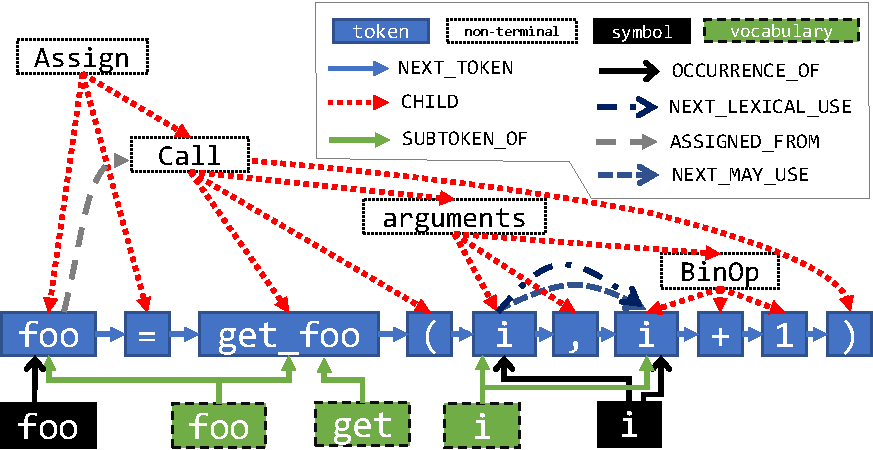
\includegraphics[width=0.75\columnwidth]{figures/samplegraph.pdf}
    \caption{Sample graph for foo=get\_foo(i, i+1) showing different node and edge types implemented by Allamanis et al.~\cite{allamanis2020typilus}.}
    \label{fig:samplegraph}
\end{figure}

The source files are processed to generate graphs that contain AST, DFG, as well as lexical and syntactical information.
An example of such a graph is shown on Figure~\ref{fig:samplegraph}.
In addition to extracting graphs from source code AST, we split them by setting a maximum node and edges number in one graph.
For this, we prune the graphs around nodes that have annotations that are later used as targets during training and testing.
Finally, we split the data into train-validation-test sets with proportions of 70-10-20, respectively.

\subsection{Model Architecture}\label{subsec:model-architecture}

We base our model architecture on TokenGT~\cite{kim_pure_2022}.
The main advantage of this model is that standard Transformer architecture is not altered to support graph data.
It allows us to use some advantages developed specifically for Transformers.
For instance, Performer~\cite{choromanski_rethinking_2020} is used to speed up training by using linear time as space complexity.

The main idea of the authors is that combining appropriate token-wise embeddings and self-attention over the node and edge tokens
is expressive enough to accurately encode graph structure to make graph and node-wise predictions.
The embeddings in the model are composed of orthonormal node identifiers, namely Laplacian eigenvectors obtained from
eigendecomposition of graph Laplacian matrix.
In addition, type identifiers are used to encode types of tokens (nodes or edges).

In our model, we use node and edge types extracted from code as token features.
Node ground truth annotations are added to the features and randomly masked during training.
The overall architecture of the model is displayed at Figure~\ref{fig:model}.

\subsubsection{Masked Transformer Encoder Model}

\begin{figure*}[t]
    \resizebox{\textwidth}{!}{\begin{tikzpicture}[
code/.style={},
v1/.style={circle,fill=WildStrawberry,minimum size=16pt},
v2/.style={circle,fill=Peach,minimum size=16pt},
v3/.style={circle,fill=VioletRed,minimum size=16pt},
v4/.style={circle,fill=DarkOrchid,minimum size=16pt},
e1/.style={draw,line width=4pt,-,Emerald},
e2/.style={draw,line width=4pt,-,SpringGreen},
e3/.style={draw,line width=4pt,-,SpringGreen!50},
e4/.style={draw,line width=4pt,-,Emerald!50},
arrow/.style={draw,->,black},
dashed arrow/.style={dashed,draw,->,black},
identifier/.style={align=center,font=\small},
rounded/.style={rectangle,minimum size=16pt,rounded corners=4pt},
vi/.style={rounded,fill=RoyalBlue},
ei/.style={rounded,fill=RoyalBlue!50},
*|/.style={
    to path={
        (perpendicular cs: horizontal line through={(\tikztostart)},
        vertical line through={(\tikztotarget)})
        % is the same as (\tikztostart -| \tikztotarget)
        % but just to be safe: http://tex.stackexchange.com/a/29781/16595
        -- (\tikztotarget) \tikztonodes
    }
},
]

% Source code
\node[code,label={[font=\small]below:Source code}] (code) {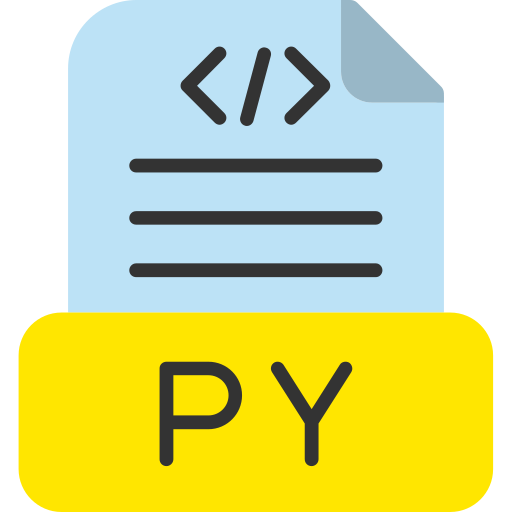
\includegraphics[width=30pt,keepaspectratio]{assets/py_code.png}};

% AST Graph
\node[v1,label=above:$V1$,right=40pt of code,yshift=-15pt] (v1) {};
\node[v2,label=above:$V2$,above right=20pt and 20pt of v1] (v2) {};
\node[v3,label=above:$V3$,right=40pt of v1] (v3) {};
\node[v4,label=above:$V4$,above right=20pt and 20pt of v3] (v4) {};

\path[e1] (v1) -- (v2);
\path[e2] (v2) -- (v4);
\path[e3] (v3) -- (v2);
\path[e4] (v4) -- (v3);

\node[fit=(v1) (v2) (v3) (v4),label={[font=\small]below:AST Graph}] (graph) {};

\path[arrow] (code) -- (graph);

% Identifiers
\node[identifier,above right=30pt and 12pt of v4] (ti) {Type\\Identifiers};

\node[vi,right=25pt of ti,label={[font=\small]below:[node]}] (v) {v};
\node[ei,right=10pt of v,label={[font=\small]below:[edge]}] (e) {e};

\node[below=10pt of ti,identifier] (ni) {Node\\Identifiers};

\node[v1,rounded,right=5pt of ni] (n1) {1};
\node[v2,rounded,right=5pt of n1] (n2) {2};
\node[v3,rounded,right=5pt of n2] (n3) {3};
\node[v4,rounded,right=5pt of n3] (n4) {4};

\path[draw,decorate,decoration={brace,mirror,amplitude=5pt,raise=2pt}] (n1.south) -- (n4.south) node[midway,below=5pt,font=\small] (orthnormal) {orthonormal};

    {[on background layer]
\node[fit=(ti) (ni) (v) (e) (n1) (n2) (n3) (n4) (orthnormal),fill=Gray!20,above right=-20pt and 10pt of v4,minimum size=60pt,rounded corners=4pt] (identifiers) {};
}

\path[dashed arrow] (graph) |- (identifiers);

\path[draw,->,black] (n4)+(15pt,0) -- +(35pt,0);
\path[draw,->,black] (e)+(33pt,0) -- +(53pt,0);

% V1

\node[v1,rounded,right=40pt of n4.north,yshift=0.5pt] (nt1-1) {1};
\node[v1,rounded,below=1pt of nt1-1] (nt1-2) {1};

    {[on background layer]
\node[fit=(nt1-1) (nt1-2),rounded corners=4pt,rectangle,draw=black] (nt1) {};
}

\node[vi,above=10pt of nt1-1] (vi-1) {v};

\node[v1,below=27pt of nt1-1] (v1-1) {};

\path[draw,->,black] (graph.center)+(35pt,-5pt) -- (332pt,-5pt) node[midway,below=5pt,font=\small] (mask) {Randomly masked type annotations};

    {[on background layer]
\path[draw,->,black] (v1-1) -- +(0,95pt);
}

% E1

\node[v1,rounded,right=10pt of nt1-1] (nt2-1) {1};
\node[v2,rounded,below=1pt of nt2-1] (nt2-2) {2};

    {[on background layer]
\node[fit=(nt2-1) (nt2-2),rounded corners=4pt,rectangle,draw=black] (nt2) {};
}

\node[ei,above=10pt of nt2-1] (ei-1) {e};

\node[below=27pt of nt2-1,opacity=0.0,minimum size=16pt,rectangle] (e1-1-tmp) {};
\node[fill=Emerald,below=27pt of nt2-1,node distance=10pt,minimum width=4pt,minimum height=16pt,rectangle,inner sep=0,rotate around={135:(e1-1-tmp.center)}] (e1-1) {};

    {[on background layer]
\path[draw,->,black] (e1-1) -- +(0,95pt);
}

% V2

\node[v2,rounded,right=10pt of nt2-1] (nt3-1) {2};
\node[v2,rounded,below=1pt of nt3-1] (nt3-2) {2};

    {[on background layer]
\node[fit=(nt3-1) (nt3-2),rounded corners=4pt,rectangle,draw=black] (nt3) {};
}

\node[vi,above=10pt of nt3-1] (vi-2) {v};

\node[v2,semicircle,minimum size=8pt,below=30.5pt of nt3-1,node distance=10pt] (v2-1) {};

    {[on background layer]
\path[draw,->,black] (v2-1) -- +(0,95pt);
}

% E2

\node[v2,rounded,right=10pt of nt3-1] (nt4-1) {2};
\node[v3,rounded,below=1pt of nt4-1] (nt4-2) {3};

    {[on background layer]
\node[fit=(nt4-1) (nt4-2),rounded corners=4pt,rectangle,draw=black] (nt4) {};
}

\node[ei,above=10pt of nt4-1] (ei-2) {e};

\node[below=27pt of nt4-1,opacity=0.0,minimum size=16pt,rectangle] (e2-1-tmp) {};
\node[fill=SpringGreen!50,below=27pt of nt4-1,node distance=10pt,minimum width=4pt,minimum height=16pt,rectangle,inner sep=0,rotate around={45:(e2-1-tmp.center)}] (e2-1) {};

    {[on background layer]
\path[draw,->,black] (e2-1) -- +(0,95pt);
}

% V3

\node[v3,rounded,right=10pt of nt4-1] (nt5-1) {3};
\node[v3,rounded,below=1pt of nt5-1] (nt5-2) {3};

    {[on background layer]
\node[fit=(nt5-1) (nt5-2),rounded corners=4pt,rectangle,draw=black] (nt5) {};
}

\node[vi,above=10pt of nt5-1] (vi-3) {v};

\node[v3,semicircle,minimum size=8pt,below=30.5pt of nt5-1,node distance=10pt] (v3-1) {};

    {[on background layer]
\path[draw,->,black] (v3-1) -- +(0,95pt);
}

% E3

\node[v3,rounded,right=10pt of nt5-1] (nt6-1) {3};
\node[v4,rounded,below=1pt of nt6-1] (nt6-2) {4};

    {[on background layer]
\node[fit=(nt6-1) (nt6-2),rounded corners=4pt,rectangle,draw=black] (nt6) {};
}

\node[ei,above=10pt of nt6-1] (ei-3) {e};

\node[below=27pt of nt6-1,opacity=0.0,minimum size=16pt,rectangle] (e3-1-tmp) {};
\node[fill=Emerald!50,below=27pt of nt6-1,node distance=10pt,minimum width=4pt,minimum height=16pt,rectangle,inner sep=0,rotate around={135:(e3-1-tmp.center)}] (e3-1) {};

    {[on background layer]
\path[draw,->,black] (e3-1) -- +(0,95pt);
}

% V4

\node[v4,rounded,right=10pt of nt6-1] (nt7-1) {4};
\node[v4,rounded,below=1pt of nt7-1] (nt7-2) {4};

    {[on background layer]
\node[fit=(nt7-1) (nt7-2),rounded corners=4pt,rectangle,draw=black] (nt7) {};
}

\node[vi,above=10pt of nt7-1] (vi-4) {v};

\node[v4,below=27pt of nt7-1,node distance=10pt] (v4-1) {};

    {[on background layer]
\path[draw,->,black] (v4-1) -- +(0,95pt);
}

% E3

\node[v4,rounded,right=10pt of nt7-1] (nt8-1) {4};
\node[v2,rounded,below=1pt of nt8-1] (nt8-2) {2};

    {[on background layer]
\node[fit=(nt8-1) (nt8-2),rounded corners=4pt,rectangle,draw=black] (nt8) {};
}

\node[ei,above=10pt of nt8-1] (ei-4) {e};

\node[below=27pt of nt8-1,opacity=0.0,minimum size=16pt,rectangle] (e4-1-tmp) {};
\node[fill=SpringGreen,below=27pt of nt8-1,node distance=10pt,minimum width=4pt,minimum height=16pt,rectangle,inner sep=0,rotate around={90:(e4-1-tmp.center)}] (e4-1) {};

    {[on background layer]
\path[draw,->,black] (e4-1) -- +(0,95pt);
}


\path (v2-1) -- (e3-1) node[identifier,midway,below=12pt] (embeddings) {Node and Edge Tokens\\with Token-wise Embedding};

% Transformer

\node[fit=(nt1-1) (nt1-2) (nt2-1) (nt2-2) (nt3-1) (nt3-2) (nt4-1) (nt4-2) (nt5-1) (nt5-2) (nt6-1) (nt6-2) (nt7-1) (nt7-2) (nt8-1) (nt8-2),fill=Gray!20,rounded,draw,label=center:Transformer Encoder + MLP,above=20pt of vi-1,anchor=south west,xshift=-12pt] (transformer) {};

% Prediction

\node[v2,above=80pt of vi-2] (vp-2) {};
\node[v3,above=80pt of vi-3] (vp-3) {};

\path[draw,->,*|,black,shorten >=2pt] (transformer.north) to (vp-2);

\path[draw,->,*|,black,shorten >=2pt] (transformer.north) to (vp-3);

\path (vp-2) -- (vp-3) node[identifier,midway,above=12pt] (embeddings) {Type annotation predictions};


\end{tikzpicture}}
    \caption{GraphTyper Architecture. The source code is first transformed into AST graph, then type annotations are randomely masked. The graph is enriched by token type identifiers (node or edge) and orthonormal node identifiers obtained from eigendecomposition of Laplacian matrix. The resulting graph is fed through a Transformer Encoder to obtain type annotations for masked nodes.}
    \label{fig:model}
\end{figure*}

Predicting type annotations in graph domain is a node classification task.
However, since we are using a Pure Transformer with graphs represented as a sequence of tokens, the task can be reduced to token classification.
In the Natural Language Processing (NLP) domain, this is a ubiquitous task, also known as Named Entity Recognition (NER).

Encoder-only architecture has been widely used for the NER task, namely BERT is one of the most popular models~\cite{liu2021nerbert,Darji_2023}.
We adapt similar architecture by randomly masking type annotations.
We then apply an MLP layer to the output of TokenGT~\cite{kim_pure_2022} to get logits of type annotations.

Masked model architecture is very versatile, and the pretrained model can be later easily fine-tuned for other tasks,
similar to the approaches from the NLP-domain~\cite{liu2021nerbert}.
For example, error~\cite{bieber2022static} and vulnerability~\cite{sun2023exploring} data can be added to the code graph to detect and fix them~\cite{nguyen_regvd_2021,li_vuldeepecker_2018,cao_bgnn4vd_2021,li_sysevr_2021,russell_automated_2018}.